\documentclass[11pt,a4paper]{article}
\usepackage[utf8]{inputenc}
\usepackage[T1]{fontenc}
\usepackage{lmodern}
\usepackage[ngerman]{babel}
\usepackage{graphicx}
\usepackage{babelbib}
\usepackage{hologo}
\usepackage{csquotes}
\usepackage{amsmath}
\usepackage{amssymb}
\usepackage{amsthm}

\begin{document}

\section{Deckblatt}
\section{Inhaltsverzeichnis}



\section{Zusammenfassung}

\section{Einleitung}
\label{sec:einleitung}
Die vorliegende Arbeit soll einen Überblick über das Container-Orchestrierungs-Tool \emph{Kubernetes} geben. 
Dazu werden zunächst Historie und grundlegende Funktionsprinzipien von Kubernetes beschrieben, die anschließend
anhand einer beispielhaften Anwendung aus dem Bereich verteilter, agentenbasierter Simulationen demonstriert werden.

Zunächst soll die Historie betrachtet werden, vor deren Hintergrund Kubernetes entstanden ist.
Das stetige Ziel, das in sich durch diese Historie zieht, ist das Bereitstellen von Applikationen.
Kominos et al. \cite{7899247} beschreiben die 1960er Jahre als Ursprung des Cloud Computing.
Zu dieser Zeit liefen Applikationen oft auf einer gemeinsamen Hardware und die Ressourcenverteilung erfolgte unmittelbar durch das zugrundeliegende Betriebssystem.
Ein derartiges Szenario (auch als ``Bare-metal`` bezeichnet) bringt in der Regel mehrere Herausforderungen mit sich.
Zum einen kann es schnell zu Abhängigkeitskonflikten zwischen den verschiedenen Applikationen geben.
Ist eine Applikation darauf angewiesen eine bestimmte Abhängigkeit in der Version <1.4 zu nutzen und eine andere
benötigt eine Version \(\geq 1.4\) derselben Abhängigkeit, lässt sich das nur schwer vereinbaren.
Zum anderen erschwert dieser Aufbau eine effiziente Ressourcenverteilung. Selbst wenn eine Applikation alleine auf einem Rechner betrieben wird (z.B. um Konflikte zu anderen
Applikationen zu vermeiden), muss dieser Rechner ausreichende Kapazitäten haben, um die höchsten Anfragespitzen an diese Applikation zu verarbeiten.
Selbst dann wenn diese Anfragespitzen nur äußerst selten erreicht werden.

Eine Weiterentwicklung dieser Bare-metal-Architektur waren virtuelle Maschinen. Virtuelle Maschinen erlauben es, auf derselben Hardware mehrere virtuelle Instanzen eines
Systems zu nutzen. Die Instanzen nutzen dabei nicht direkt die physischen Ressourcen, sondern lediglich virtuelle, die durch Software nachgebildet werden \cite{kofler2021docker}.
Dadurch, dass verschiedene Applikationen in verschiedenen virtuellen Maschinen betrieben werden, können Abhängigkeitskonflikte zwischen Applikationen
vermieden werden. Weiterhin sind virtuelle Maschinen leichter auszubringen und zu administrieren als Bare-metal-Lösungen.
Grundsätzlich können mit diesem Ansatz Applikationen auch flexibler und skalierbarer bereitgestellt werden.
Leistungsfähige Hardware kann Anfragespitzen einer Applikation in einer virtuellen Maschine abfangen und zu anderen Zeiten anderen virtuellen Maschinen mit anderen
Applikationen diese Ressourcen zuweisen.
Obwohl das schon einige Verbesserungen im Vergleich zu Bare-metal-Lösungen sind, haben auch virtuelle Maschinen ihre eigenen Limitationen.
Da virtuelle Maschinen jeweils Ressourcen für ein eigenes Betriebssystem beanspruchen, geht vergleichsweise viel Leistung verloren, 
die besser in der Applikation genutzt werden könnte.

Die nächste Stufe der Weiterentwicklung waren (Software-)Container. Container haben einige Gemeinsamkeiten mit virtuellen Maschinen, doch der wesentliche Unterschied ist,
dass Container deutlich leichtgewichtiger sind. Das wird unter anderem dadurch erreicht, dass sie statt ein komplett eigenes Betriebssystem zu verwenden, 
Anteile des Host-Betriebssystems mitnutzen. Dadurch sind die ``Baupläne`` (sog. Images) für Container im Allgemeinen kleiner als für klassische virtuelle Maschinen.
Durch den verringerten Overhead können auf gleicher Hardware auch mehr Container parallel betrieben werden, als es mit virtuellen Maschinen möglich wäre.
Durch diesen Umstand und dadurch, dass Container meist innerhalb weniger Sekunden gestartet werden können, sind diese besonders geeignet,
um flexibel auf unterschiedliche Anfrageintensitäten zu reagieren und Ressourcen effizient zu verteilen \cite{kofler2021docker}.

Einzelne Container führen in der Regel nur eine klar umgrenzte Aufgabe aus (z.B. Betrieb einer Datenbank oder eines Webservers). Da sie in sich geschlossen sind,
können sie auch unabhängig von anderen Containern repliziert werden. Um eine vollständige Anwendung zu erhalten, betreibt man daher oft mehrere Container,
die im Verbund zusammenwirken; eine sogenannte Microservice-Architektur. Um den hohen Anforderungen an Rechenleistung moderner Anwendungen gerecht zu werden,
werden die Container dabei oft auf viele Rechner verteilt (sog. horizontale Skalierung). % Horizontale und vertikale Skalierung noch erklären?
Die Verwaltung einer solchen verteilten Microservice-Architektur kann schnell komplex werden, weshalb verschiedene Werkzeuge zur Unterstützung entwickelt wurden.

Eines der heute populärsten Werkzeuge dieser Art ist Kubernetes. Im Folgenden soll die Funktionsweise von Kubernetes beschrieben und schließlich anhand eines Beispiels 
verdeutlicht werden.

\section{Historie von Kubernetes}
Kubernetes ist eine Software, die sich der Ausbringung (Deployment), der Skalierung und der Steuerung (Management) von Containern widmet.
Dieser Vorgang wird auch als Container-Orchestrierung oder auch Container-Management bezeichnet \cite{Bisong2019}.
In diesem Zusammehang wird Kubernetes auch als \emph{Betriebssystem der Cloud} bezeichnet \cite{Schmeling_Dargatz_2022}. 
Entwickelt wurde Kubernetes von Google. Dort wurde seit den frühen 2000er Jahren ein selbst entwickeltes Container-Management-System namens \emph{Borg} genutzt,
um Googles Services möglichst performant zu betreiben. 
Im Jahr 2013 wurd \emph{Borg} von dessen Nachfolger \emph{Omega} abgelöst. Im selben Jahr erschien auch Docker, was ein wesentlicher Baustein des Kubernetes 
Projekts werden sollte.

Die drei bei Google beschäftigten Ingenieure Craig McLuckie, Joe Beda und Brendan Burns setzten sich damals dafür ein,
die bei \emph{Borg} und \emph{Omega} gemachten Erfahrungen zu nutzen, um ein leichter bedienbares Container-Orchestrierungs-Tool 
mit nutzerfreundlicher Schnittstelle zu entwickeln.

2014 wurde Kubernetes als eine Open-Source-Variante von \emph{Borg} veröffentlicht und schließlich 2015 mit der Veröffentlichung von Kubernetes 1.0
von Google an die Cloud Native Computing Foundation (CNCF, https://www.cncf.io/) gespendet. In den folgenden Jahren wuchs der Nutzerkreis von Kubernetes
rasch an und es konnte sich deutlich gegen konkurrierende Anwendungen durchsetzen.

Heutzutage ist Kubernetes, nach Linux, das zweitgrößte Open-Source Projekt der Welt und wird von 71\% der Fortune 100 Unternehmen genutzt. % (https://www.cncf.io/reports/kubernetes-project-journey-report/)
% https://www.ibm.com/think/topics/kubernetes-history abgerufen am 28.11.2024

\section{Container}

Um den Begriff des (Docker-)Containers zu verstehen, wird zunächst der Begriff \emph{Image} benötigt.
Ein Image kann wie in der Einleitung bereits beschrieben als eine Art Bauplan für einen Container gesehen werden.
Es stellt ein read-only Dateisystem als Basis für den Container zur Verfügung. Der Container nimmt an seinem Image
keine Änderungen vor. Stattdessen wird jedes Hinzufügen und jede Änderung während der Laufzeit des Containers in einem
getrennten Overlay-System behandelt. Dadurch können beliebig viele Container von demselben Image abgeleitet werden \cite{kofler2021docker}. 

Für viele populäre Anwendungen (z.B. nginx, ubuntu oder nodejs) gibt es vorgefertigte Images, die kostenfrei vom DockerHub % Quelle ergänzen
heruntergeladen werden können.
Für einen konkreten Anwendungsfall kann es sinnvoll sein, ein bestehendes Basis-Image für die eigenen Zwecke anzupassen.
Dies ist mit Hilfe eines sogenannten \emph{Dockerfile}s möglich. Darin wird definiert, wie ein Base-Image z.B. durch das Hinzufügen von Dateien,
oder dem Ändern von Umgebungsvariablen angepasst werden soll. Dieses \emph{Dockerfile} wird dann für den \emph{build}
eines neuen Images verwendet.
% Bild von Workflow einbinden?

Aus dem erstellten Image können dann Container abgeleitet werden. Ein Container ist insofern ``flüchtig`` als dass er nach seiner
Beendigung restlos gelöscht wird. Bei einem Neustart enthält er wieder nur die Daten, die vorher durch das Image definiert wurden.
Natürlich gibt es Anwendungsfälle, in denen die persistente Speicherung von Daten durch einen Container gewünscht ist, z.B. wenn
eine Datenbank in einem Container betrieben wird. Für diesen Fall gibt es das Konzept der \emph{Volumes}.
Ein Volume spiegelt einen definierten Speicherbereich aus dem Dateisystem des Containers auf das Host-System. 
Wird ein Container beendet und durch einen neuen ersetzt, bindet dieser das Volume in sein Dateisystem ein übernimmt dabei die Daten seines beendeten Vorgängers.

Die in diesem Abschnitt beschriebenen Konzepte sind ausreichend, um Container zu betreiben.
Nutzt man aber lediglich diese Konzepte, verhalten sich die Container im Prinzip wie leichtgewichtige virtuelle Maschinen.
Der eigentliche Vorteil von Containern, nämlich die horizontale Skalierbarkeit, wird damit noch nicht ausgenutzt.

Bie horizontale Skalierbarkeit ist abzugrenzen von der vertikalen Skalierbarkeit. Bei letzterer geht es darum, den Computer, der eine Anwendung betreibt,
um weitere Rechen- oder Speicherressourcen zu erweitern. Dieser Ansatz ist zwar leichter zu administrieren, da keine Änderungen an der Anwendung selbst
erforderlich sind, aber er stößt auch bald an seine physikalischen Grenzen. Horizontale Skalierung sieht im Gegensatz dazu vor, dass eine Anwendung
auf mehrere Rechner verteilt wird. Durch Hinzufügen weiterer Rechner können die zur Verfügung stehenden Ressourcen nahezu beliebig erweitert werden.
Zusätzlich ist auch eine geografische Optimierung möglich, indem zum Beispiel Server in der Nähe der erwarteten Clients platziert werden. 
Letztendlich trägt horizontale Skalierung auch zur Ausfallsicherheit einer Anwendung bei, da der Ausfall einzelner Instanzen durch andere Instanzen
aufgefangen werden kann.
Der Nachteil dieser Methode ist die deutliche erhöhte Komplexität, die mit dem Betrieb einer verteilten Anwendung einhergeht.

Im folgenden Abschnitt soll beschrieben werden, welche Werkzeuge Kubernetes anbietet, um mit dieser Komplexität umzugehen.

\section{Grundlegende Kuberneteskonzepte}
Ein durch Kubernetes verwaltetes System wird üblicherweise als \emph{Cluster} bezeichnet.
Ein Cluster besteht aus einer oder mehreren physischen und/oder virtuellen Maschinen, die darin eingebunden sind.
Jede Maschine wird dabei als ein \emph{Node} (deutsch: Knoten) bezeichnet. Diese Nodes werden wiederrum unterschieden in 
\emph{Master Nodes} und \emph{Worker Nodes}.
Für die meisten Cluster reicht ein Master Node aus. In Hochverfügbarkeitsszenarien oder bei mehreren
tausend Worker Nodes kann es jedoch auch mehrere Master Nodes geben \cite{Schmeling_Dargatz_2022}.
Wie die Namen vermuten lassen, ist der Master Node dafür verantwortlich für die Orchestrierung
des Systems verantwortlich während die Worker Nodes bestimmte Aufgaben ausführen \cite{Bentaleb_Belloum_Sebaa_El-Maouhab_2021}.
Für den Spezialfall eines \emph{Single-Node-Clusters} kann dieser einzelne Node auch die Rolle von sowohl
Master als auch Worker übernehmen.
Master und Worker Nodes bestehen zur Erfüllung ihrer Aufgaben aus unterschiedlichen Komponenten,
die im folgenden beschrieben werden.

\subsection{Master Node Komponenten}
\subsubsection{Etcd}
Bei \emph{Etcd} handelt es sich um einen \emph{key-value-store} (Schlüssel-Wert-Speicher),
der alle Informationen über den Zustand eines Kubernetes Clusters speichert.
Jede Änderung an den Cluster-Ressourcen wird im Etcd gespeichert und von dort wieder abgerufen.
Etcd wird auf jedem Master Node ausgeführt, wobei einer dieser Nodes als ``Anführer`` 
ausgewählt wird und dieser die Schreibanfragen verarbeitet.

\subsubsection{Kube-apiserver}
Die übliche Vorgehensweise um mit einem Kubernetes Cluster zu interagieren, ist das Kommandozeilenwerkzeug \emph{kubectl}.
Dieses Werkzeug ermöglicht sowohl die Abfrage als auch die Änderung von im Cluster vorhandenen Ressourcen.

Im Hintergrund stellt \emph{kubectl} eine Anfrage an den Kube-apiserver, der Endpunkte anbietet, 
um mit dem Cluster zu interagieren. Der Kube-apiserver ist somit dafür verantwortlich, die angefragen Informationen,
aus verschiedenen Quellen zu sammeln und gegebenenfalls andere Komponenten anzuweisen, bestimmte Änderungen vorzunehmen.

\subsubsection{Kube-Controller-Manager}
Neben dem tatsächlichen Zustand des Clusters enthält Etcd auch den gewünschten Zustand.
Sollten diese voneinander abweichen, ist es die Aufgabe des Kube-Controller-Managers,
dies zu erkennen und über eine Anfrage an den Kube-apiserver den gewünschten Zustand wiederherzustellen.


\subsubsection{Kube-Scheduler}
Der Kube-Scheduler entscheidet, welche Container auf welchem Node betrieben werden.
Er verwaltet dazu Informationen über verfügbare Rechen- und Speicherressourcen sowie weiterer Eigenschaften
der Nodes. 
\subsection{Worker Node Komponenten}

Auf jedem Worker Node finden sich drei wesentliche Komponenten.
Die erste Komponente ist der \emph{Kubelet}. Das Kubelet kann als Schnittstelle
zu den Master Nodes gesehen werden. Sobald der Kube-Scheduler entschieden hat, auf welchem
Worker Node ein Container betrieben werden soll, bekommt das Kubelet auf diesem Node 
vom Kube-apiserver den Auftrag einen Container zu starten.

Kubelet gibt diesen Auftrag weiter an die Komponente \emph{Container Runtime}.
Diese übernimmt das eigentliche Starten des Containers, in dem sie das zugehörige Image
abruft (z.B. von DockerHub) und daraus einen Container erstellt.

Der physische ``Standort`` eines Containers, also der Node, auf dem er betrieben wird, ist insofern
flüchtig, als dass der Container jederzeit auf einem anderen Node neu ausgebracht werden könnte.
Um trotzdem einen Überblick zu behalten, welcher Container wo verortet ist, gibt es die Komponente
\emph{Kube-Proxy}. Auf jedem Node läuft genau eine Instanz des Kube-Proxy.

Eine ausführlichere Erläuterung der oben aufgeführten Komponenten kann bei Schmeling und Dargatz \cite{Schmeling_Dargatz_2022}
gefunden werden.

\subsection{Pods}
\subsection{ReplicaSets}
\subsection{Deployments}
\subsection{Services}
\subsection{Ingress}
\subsection{Flottensimulation}
\subsection{Volumes}
\subsection{ConfigMaps und Secrets}
% \subsection{Namespaces?}
% Vorstellung der realen Problemstellung (Hohe Kosten für Betrieb (s. auch 10408594 S. 1), Vorhersage von effizientem Ressourceneinsatz)

% Motivation für Simulationen 
% Voraussetzung für Simulation (System- und Datenanalyse)
% Herausforderungen bei Simulationen (Hohe Anzahl an möglichen Parameterkombinationen)

\section{Flottensimulation}
\begin{figure}
	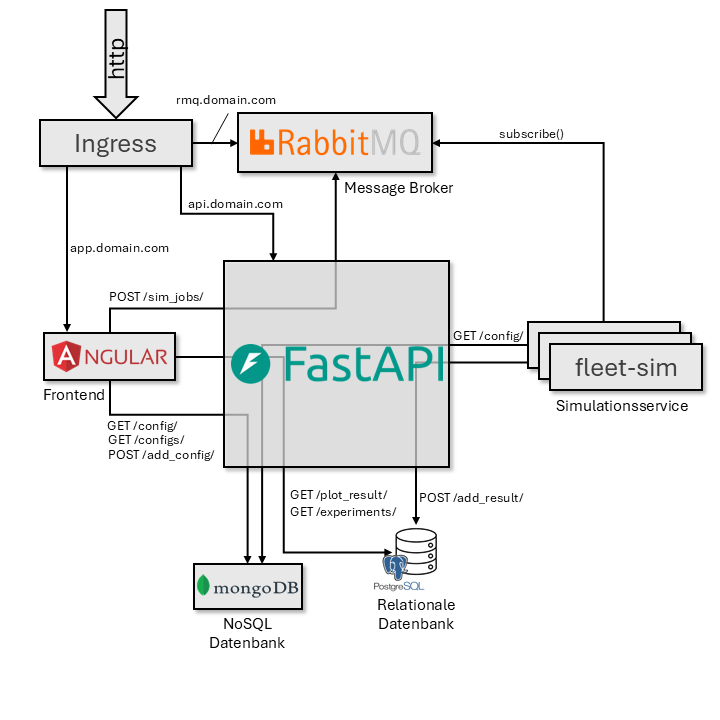
\includegraphics[width=\textwidth]{media/Microservice-Architektur.png}
\end{figure}




\subsection{Schritte zum Aufsetzen und zum Betrieb der Flottensimulation}
% \begin{enumerate}
% 	\item Wie entstand Kubernetes (Historie Google)
% 	\item Was ist ein Container? \cite{Bentaleb_Belloum_Sebaa_El-Maouhab_2021}
% 	\item Grundprinzipen/Elemente von Kubernetes (Pods, Deployments, Replicasets etc.)
% 	\item Kubernetes Workflow (allgemein)
% 	\item Nachteile verteilter Services (s. 86ff. in Schmeling\_Dargatz\_2022)
% 	\item Kubernetes anhand eines realen Beispiels
% \end{enumerate}

\section{Limitationen}
% Begrenzte Hardware und hohe Kosten bei Cloud Providern 

\section{Fazit}

\section{Ausblick}
% Nutzung einer anderen Cluster Engine als minikube (s. auch 10408202 für Rancher Alternative)
% Erweiterung des Simulationsmodells um Condition based maintenance/digital twin (s. auch 10408594)
% Erhöhung der Komplexität des Modells durch weitere Input-Faktoren
% FastAPI um Authentisierung ergänzen
\section{Anhang}


\section{Formatbeispiele}
\subsection{Eine Aufzählung}

\begin{enumerate}
	\item die \textbf{original PDF Vorlage} (also diese Datei),
	\item das von Ihnen erstellte \textbf{\hologo{LaTeX} Dokument} (also die .tex Datei),
	\item die von Ihnen erstellte \textbf{Literatur Datenbank} (also die .bib Datei), und
	\item das von Ihnen \textbf{kompilierte Dokument} (also die erzeugte .pdf Datei).
\end{enumerate}


\subsection{Tabellen}
Tabelle \ref{HdRTab} gibt eine kleine Übersicht über verschiedene Charaktere und Gruppierungen in \emph{Der Herr der Ringe}.

\begin{table}[b]
	\begin{tabular}{|r|c|c|c|c|}
		\hline
				& Gollum	& Legolas	& Sauron	& Gandalf \\
		\hline
		\hline
		Hobbit	& ja	& nein	& nein	& nein \\
		\hline
		Ringträger	& am Finger	& nein	& am Finger	& in der Hand \\
		\hline
		Gemeinschaft des Ringes	& nein	& ja	& nein	& ja \\
		\hline
	\end{tabular}
	\caption{Verschiedene Charaktere und Gruppierungen in \emph{Der Herr der Ringe}.}
	\label{HdRTab}
\end{table}

\subsection{Formeln}
Die bekannten Fibonacci-Zahlen $F_n$ sind wie folgt definiert.
\newtheorem{defn}{Definition}
\begin{defn}\label{fibonacci}
	Es sei $F_1 = F_2 = 1$ und $F_n = F_{n-1} + F_{n-2}$ für $n \geq 3$.
\end{defn}
Fibonacci-Zahlen treten sowohl in der Natur als auch in vielen theoretischen Anwendungen auf. Die folgende Formel für die in Definition \ref{fibonacci} wurde von verschiedenen Mathematikern im 18. und 19. Jahrhundert entdeckt. Es sei $\phi = \frac{1 + \sqrt{5}}{2}$ (der goldene Schnitt) und $\psi = \frac{1 - \sqrt{5}}{2}$. Dann gilt
\[ \forall n \in \mathbb{N}: \quad F_n = \frac{\phi^n - \psi^n}{\sqrt{5}}. \]

\bibliographystyle{babplain-fl}
\bibliography{literature}

\end{document}